\documentclass[11pt, oneside]{article}   	% use "amsart" instead of "article" for AMSLaTeX format
\usepackage{geometry}                		% See geometry.pdf to learn the layout options. There are lots.
\geometry{a4paper}                   		% ... or a4paper or a5paper or ...letterpaper 
%\geometry{landscape}                		% Activate for rotated page geometry
%\usepackage[parfill]{parskip}    		% Activate to begin paragraphs with an empty line rather than an indent
\usepackage{graphicx}				% Use pdf, png, jpg, or eps§ with pdflatex; use eps in DVI mode
								% TeX will automatically convert eps --> pdf in pdflatex		
\usepackage{amssymb}
\DeclareGraphicsExtensions{.pdf,.png,.jpg}
\graphicspath{ {images/} }

\usepackage{hyperref}
\usepackage{subcaption}
\usepackage{amsmath}

\usepackage{framed}


\title{Connecting Nutrition, Health and Environment }
\author{Wiktor Jurkowski, Perla Troncoso Rey, Earlham Institute}
\date{25 - 26 January 2017}	 % Activate to display a given date or no date

\begin{document}
\maketitle

\tableofcontents

\listoffigures
\listoftables


\section{Introduction}

In this practice, we will look at how to explore  gene expression data (which could be extracted from microarray or RNA sequencing data). In the first part of this practical session we will see general techniques to explore the patterns or structure of the data using Principal Component Analysis, PCA, and Hierarchical Clustering. We will then look into compiling an interaction network using an online resource and how to visualise the network using Cytoscape \cite{Shannon2003} \cite{Smoot2011}.

In the second part, we will look at ways to rank genes (and/or metabolites) using approaches based on logistic regression. We will then perform pathway analysis using those rankings.

We will use a publicly available data from a study on fatty liver disease of obese and lean human subjects \cite{Wruck2015}.



\part{Part I}

\subsection{Exploring the expression data}

One could obtain gene expression from microarrays or RNA sequencing data. It is not within the scope of this session to look at the details of obtaining quantifying the expression of genes from microarrays or RNA sequencing data but instead we will start our analysis assuming that expression data has been quantified.
The gene expression data is normally stored in tabular file, representing a matrix where the columns are the samples or experiments, and the rows represent the genes. 

Example of expression data is shown in \autoref{fig:ExpressionData}. The table shows the expression of six genes in four different experiments or samples. This is, gene A has expression of 0.1 for sample 1, 0.8 for sample 2, 0.3 for sample 3, and so forth. 

\begin{figure}[!h]
	\centering
	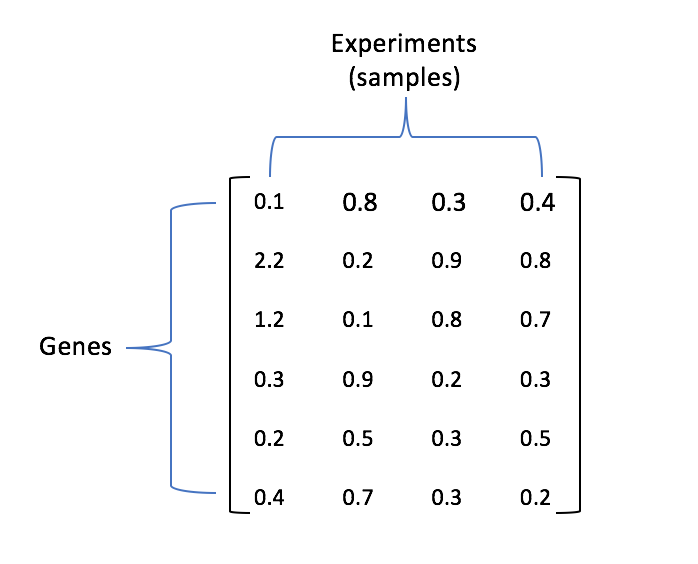
\includegraphics[width=0.7\textwidth]{example_expression_data}
	\caption{Example of expression data with samples across the columns and individual genes down the rows.}
	\label{fig:ExpressionData}
\end{figure}


Expression data can be obtained using different algorithms. One of the most well know are TopHat and Cufflinks protocol for the analysis of RNA sequencing data, which includes quantification of gene expression. \autoref{tab:ExpressionCufflinks} shows an example of the output provided by cufflinks with the estimated gene-level expression values. Cufflinks uses the notation ``XLOC\_{\it numeric\_sequence}'' to identify a gene.


\begin{table}[h]
    \centering
    \caption{Example of the output provided by cufflinks for the quantification of gene expression from RNA sequencing data.}
    \begin{tabular}{c|c|c|c|c|c|c|c|c}
    tracking\_id & sample1 & sample2 & sample3 & sample4 & sample5 & sample6 & sample7 & sample8 \\
    \hline
    XLOC\_000001 & 35.1077 & 50.9662 & 78.7724 & 35.4736 & 69.6067 & 63.9241 & 57.7967 & 61.4227 \\
    XLOC\_000002 & 49.7359 & 64.6178 & 46.8884 & 74.617 & 66.0371 & 42.9654 & 645.65 & 64.8351 \\
    XLOC\_000003 & 0 & 0 & 0.937767 & 0 & 0 & 0 & 0 & 0\\
    XLOC\_000004 & 89.7196 & 85.5504 & 185.678 & 74.617 & 142.783 & 168.718 & 172.63 & 167.206 \\
    XLOC\_000005 & 12.6778 & 39.1347 & 158.483 & 22.0181 & 28.5566 & 45.0613 & 15.9701 & 50.0481 \\
    XLOC\_000006 & 10.7273 & 9.1011 & 10.3154 & 13.4555 & 7.13915 & 6.28762 & 7.60483 & 12.512 \\
    XLOC\_000007 & 0 & 0 & 0.937767 & 0 & 0 & 0 & 0 & 0 \\
    XLOC\_000008 & 55.5871 & 37.3145 & 86.2746 & 66.0544 & 66.9295 & 53.4448 & 54.7548 & 75.0722 \\
    XLOC\_000009 & 37.0581 & 16.382 & 24.3819 & 24.4646 & 38.3729 & 15.7191 & 24.3355 & 50.0481 \\
    XLOC\_000010 & 812.352 & 483.269 & 696.761 & 748.616 & 1094.97 & 521.873 & 675.309 & 741.622 \\
    XLOC\_000011 & 0 & 0 & 0 & 0 & 0 & 1.04657 & 0.760483 & 1.13746\\
    \hline
    \label{tab:ExpressionCufflinks}
    \end{tabular}
\end{table}




\subsubsection{Principal Component Analysis}

Principal Component Analysis, commonly known as PCA, is a mathematical technique that is used to explore data, specially high-dimensional data, to extract the most important trends in the data.

When thinking of gene expression data, high dimensionality comes from the large number of dimensions of the data. This is, the result of each experiment can be thought as a kind of space, where each each feature is a coordinate in the space. There are typically thousands of genes (dimensions) and the structure of pattern in the data extends to all the dimensions. 


\paragraph{How PCA works}
\paragraph{}

The mean represents the average of the values in the data:

\begin{equation}
   \bar{{\bf X}} = \frac{1}{n} \sum_{i=1}^{n} x_i 
\end{equation}

The variance provides the the spread of the data:

\begin{equation}
   \text{Var} ({\bf X}) = \sigma^2  = \frac{1}{n-1} \sum_{i=1}^{n} ( x_i -  \bar{{\bf X}})^2
\end{equation}


For example, figure \ref{fig:MeanVariance} shows two distributions with the same mean but different variance. This means that the data points are at the same location but with a different strength. Thus, the third statistic we'll need is the covariance.

\begin{figure}[!h]
	\centering
	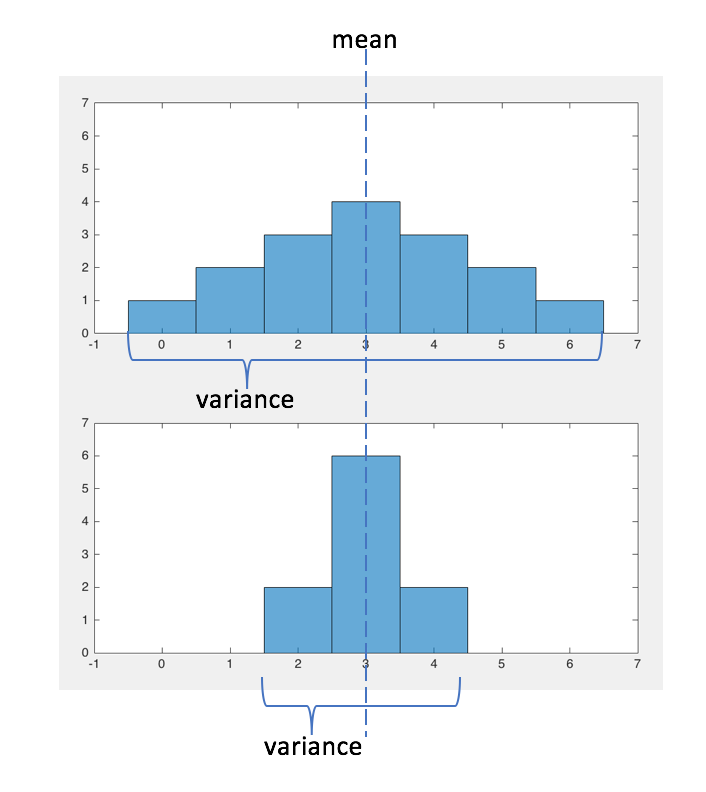
\includegraphics[width=0.7\textwidth]{same-mean_different-variance}
	\caption{Two distributions with the same mean but different variance.}
	\label{fig:MeanVariance}
\end{figure}


The covariance represents the degree of co-dependence of two variables, i.e., it measures the co-dependency of two variables, given by:

\begin{equation}
   \text{Cov} ({\bf X}, {\bf Y}) = \frac{1}{n-1} \sum_{i=1}^{n} (x_i - \bar{ {\bf X}}) (y_i - \bar{ {\bf Y}})
\end{equation}

Increases with increasing co-dependency and variance. Just as the variance measures the degree to which a set of data varies, the co-variance is a measure of the way two sets of data vary together.

\begin{equation}
   \text{Cov} ({\bf X}, {\bf X}) = \text{Var}({\bf X})
\end{equation}

The covariance also increases in magnitude as the variance of each of the two datasets increases.
Correlation values can be negative or positive, indicating whether the values of two variables increase or decrease together. Figure \ref{fig:examples-correlation} shows some examples of correlation.

\begin{figure}[!h]
	\centering
	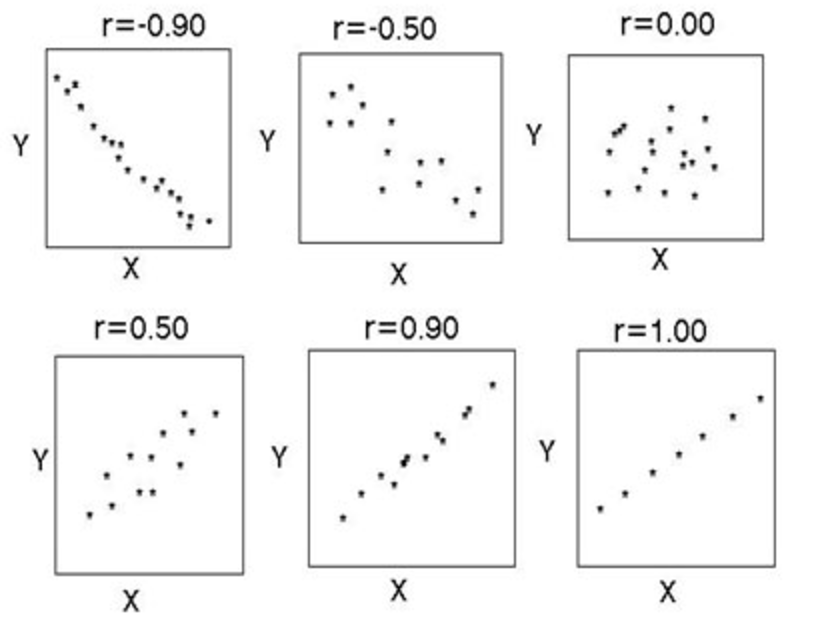
\includegraphics[width=0.7\textwidth]{examples-correlation}
	\caption{Examples of correlation}
	\label{fig:examples-correlation}
\end{figure}



\paragraph{Coordinate transformations}
\paragraph{}
In a two dimensional space described by coordinates, a point in space is described by X and Y such that ${\bf v} = [x_1, y_1]$. For example, the vector $v_1 = [1 ~2]^T$ represents the point:

An alternative coordinate systems described by the coordinates $\text{X}^\prime$ and $\text{Y}^\prime$, has a different column vector describing the same point ${\bf v^\prime} = [x_1^\prime, y_1^\prime]$.

The two coordinate systems are $T{\bf v} = {\bf v}^\prime$, related to the orthogonal transform matrix $T$ (an orthogonal matrix is the kind of matrix which performs rotated-axis coordinate transforms). 

We can make a new coordinate system by using a transformation matrix T, which relates the two coordinates vectors by matrix multiplication. There are many types of transformations but we are particularly interested in transformations which rotate the coordinate axis. These are performed by matrices which have the property called orthogonality.

\begin{figure}[!h]
	\centering
	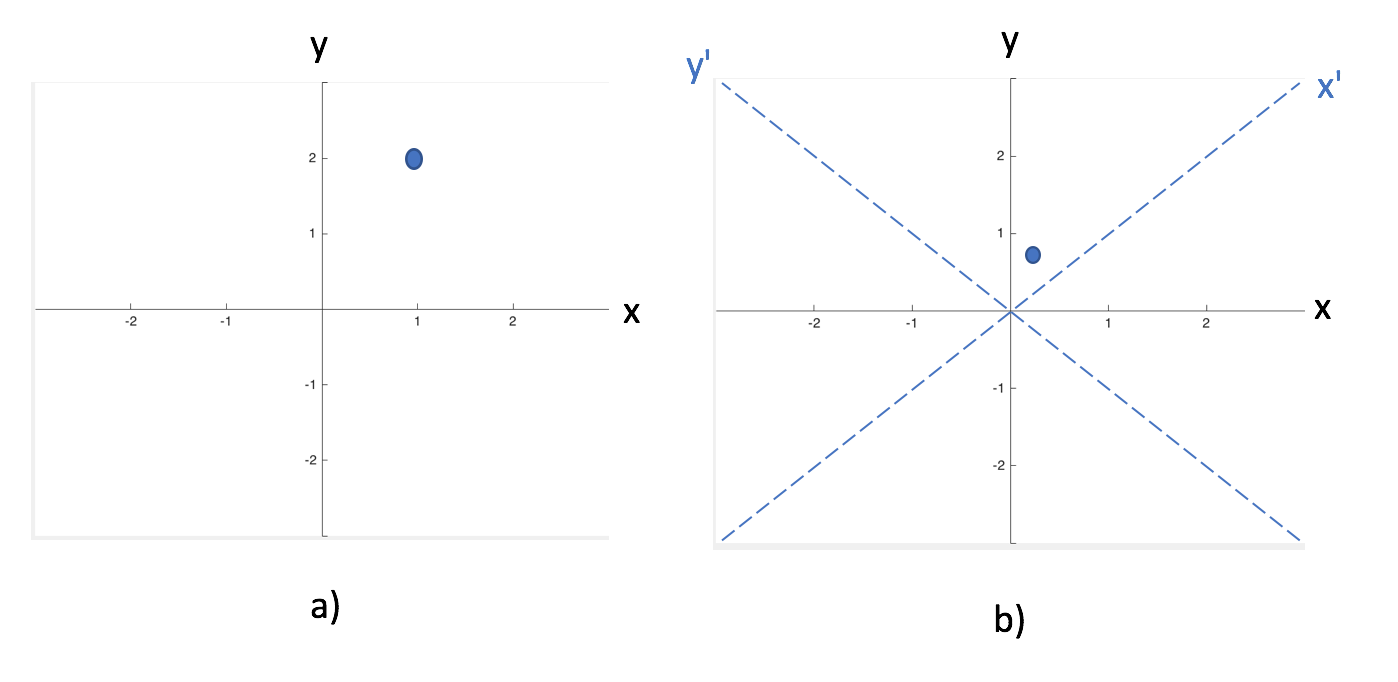
\includegraphics[width=0.7\textwidth]{example-coordinate-transform}
	\caption{Example of a coordinate transform}
	\label{fig:CoordinateTransform}
\end{figure}



\paragraph{Eigenvalues and Eigenvectors}
\paragraph{}

When a transformation matrix maps a vector to a multiple of itself, then the vector is called an Eigenvector. The amount by which the vector is multiplied (stretched) is the associated Eigenvalue:

\begin{equation}
T x = \lambda x
\end{equation} 

\noindent where $\lambda$ are the Eigenvalues and $x$ are the Eigenvectors. A matrix formed from the Eigenvectors placed in the columns is orthogonal.

In general terms, PCA uses covariants to encode the structure in the data and then eigenvectors to devise a new set of coordinates that best reveals the structure by finding the appropriate set of directions. One result from linear algebra is that if the eigenvectors are placed next to each other then the result is an orthogonal matrix that performs a coordinate transformation. This is central for PCA.

Example: 

\[ \text{The matrix: }
%
   \left(
      \begin{tabular}{cc}
      1 & 3 \\ 
      2 & 2
      \end{tabular}
   \right)
   %
   \text{has eigenvalues 4 and -1.}
   \text{ and the eigenvectors}
   \left( \begin{array}{c}
      1 \\ 
      1
      \end{array}
   \right)
   \text{and} 
   \left( \begin{array}{c}
      3 \\ 
      -2
      \end{array}
   \right)
\]


such that

\[ \left( \begin{array}{cc}
      1 & 3\\ 
      2 & 2
      \end{array} \right)
%
   \left( \begin{array}{c}
      1 \\ 
      1
      \end{array} \right)
%
   = 4
   \left( \begin{array}{c}
   1\\
   1
   \end{array} \right)
\text{~~~and~~~}
   \left( \begin{array}{cc}
   1 & 3\\
   2 & 2
   \end{array} \right)
%
   \left( \begin{array}{c}
   3\\
   -2
   \end{array} \right)
%
   =-1
   \left( \begin{array}{c}
   3\\
   -2
   \end{array} \right)
\]



\paragraph{In summary, PCA benefits are:}

\begin{itemize}

   \item A powerful tool to visualise high dimensional data 

   \item Shows quantified difference among observations

   \item Used to assess data quality and discover relationships between data points
   
   \item Some software to compute PCA is available in MATLAB and R (using package stats)

\end{itemize}




% Here we start with some hands-on exercises

% Example 1
\paragraph{Example 1: PCA for the expression of two genes}
\paragraph{}

We will use R and the package stats to perform PCA. We will use an example data which represents several measurements of the expression of two genes, $x$ and $y$, with the following values:

\begin{center}
\begin{tabular}{c|c}
   x & y \\
   \hline
   2.5 & 2.4\\
   0.5 & 0.7\\
   2.2 & 2.9\\
   1.9 & 2.2\\
   3.1 & 3.0\\
   2.3 & 2.7\\
   2.0 & 1.6\\
   1.0 & 1.1\\
   1.5 & 1.6\\
   1.1 & 0.9\\
   \hline
\end{tabular}
\end{center}
   

We start by create a matrix of points in 2-d space (gene expression data) by using the following syntax:

%% create a matrix with the data from two genes
% script
% x <- c(2.5, 0.5, 2.2, 1.9, 3.1, 2.3, 2.0, 1.0, 1.5, 1.1)
% y <- c(2.4, 0.7, 2.9, 2.2, 3.0, 2.7, 1.6, 1.1, 1.6, 0.9)
% class <- c('control', 'control', 'control', 'control', 'control',
%  'case', 'case', 'case', 'case', 'case')
% ExpData <- data.frame(x = x, y = y, class = class)
	
\begin{framed}
\begin{verbatim}
   #n number of samples
   name_gene_1 <- c(values_in_sample1, ..., _value_in_sampleN) 
   #m number of genes
   name_gene_2 <- c(gene_1, gene_2, ..., gene_m)    
   samples <- c(sample1, ..., sampleN)
   # expression matrix
   Exp <- data.frame(gene1 = name_gene1, ..., geneM = name_geneM)	
\end{verbatim}
\end{framed}


Then, we plot these two genes (see figure \ref{fig:PlotTwoGenes}) using the command: 

\begin{framed}
\begin{verbatim}
   plot(x, y)
\end{verbatim}
\end{framed}


\noindent Trends are already apparent because data is simple but this is not usually the case. We then perform an statistical analysis using Principal Component Analysis. Before starting with PCA, it is best to first have centered the data with mean zero. This is, calculate the mean of each of the two variables and substracted to obtain centered data (shown in figure \ref{fig:PlotTwoGenesCentered}). 


%Plot data and data centered
\begin{figure}[!h]
	\centering
	\begin{subfigure}{.45\textwidth}
		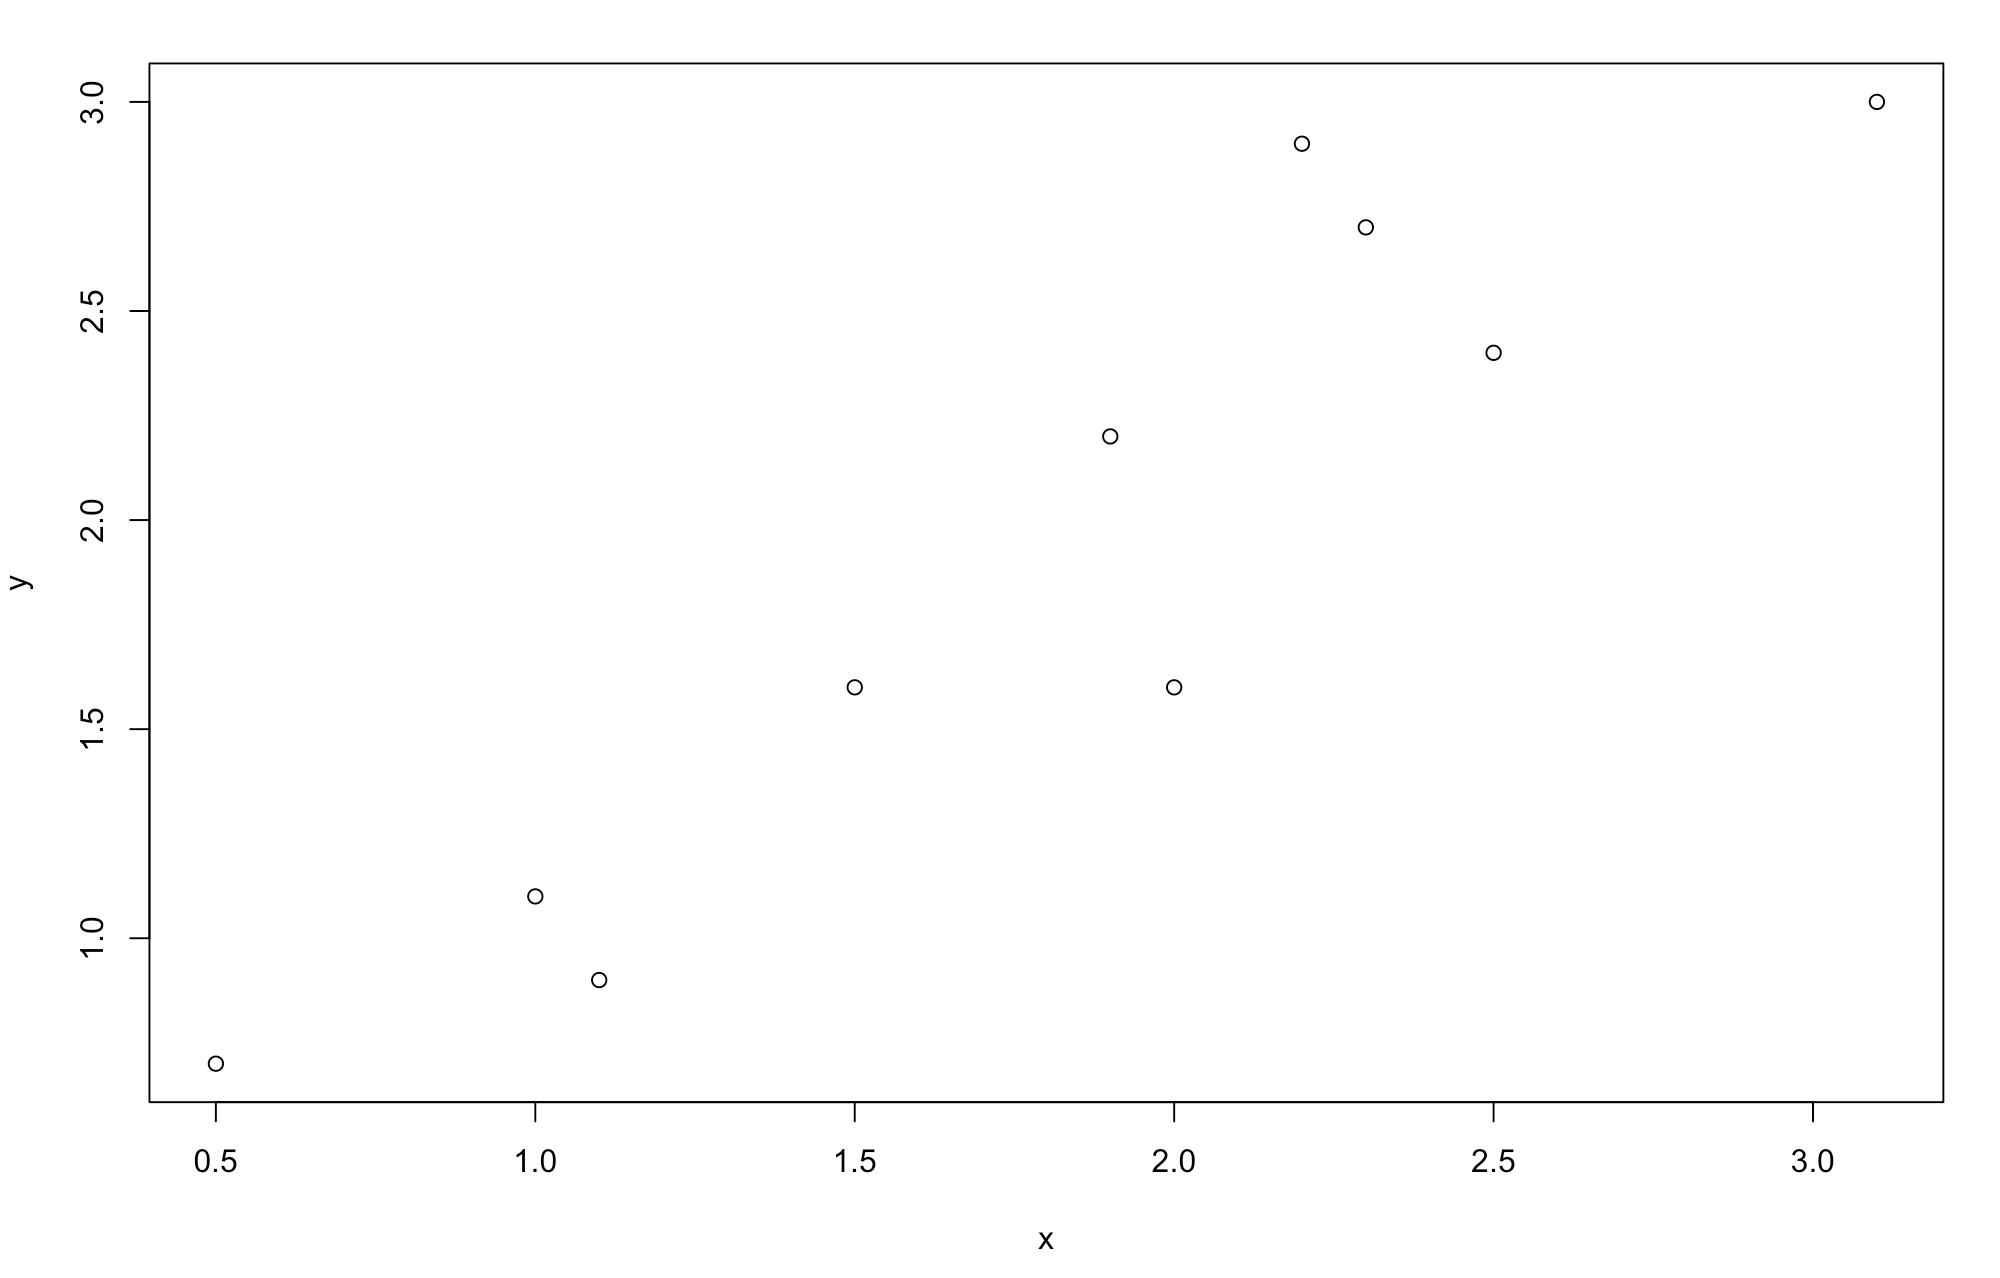
\includegraphics[width=\textwidth]{example1-plot-two-genes}
		\caption{}
		\label{fig:PlotTwoGenes}
	\end{subfigure}
	\begin{subfigure}{0.45\textwidth}
		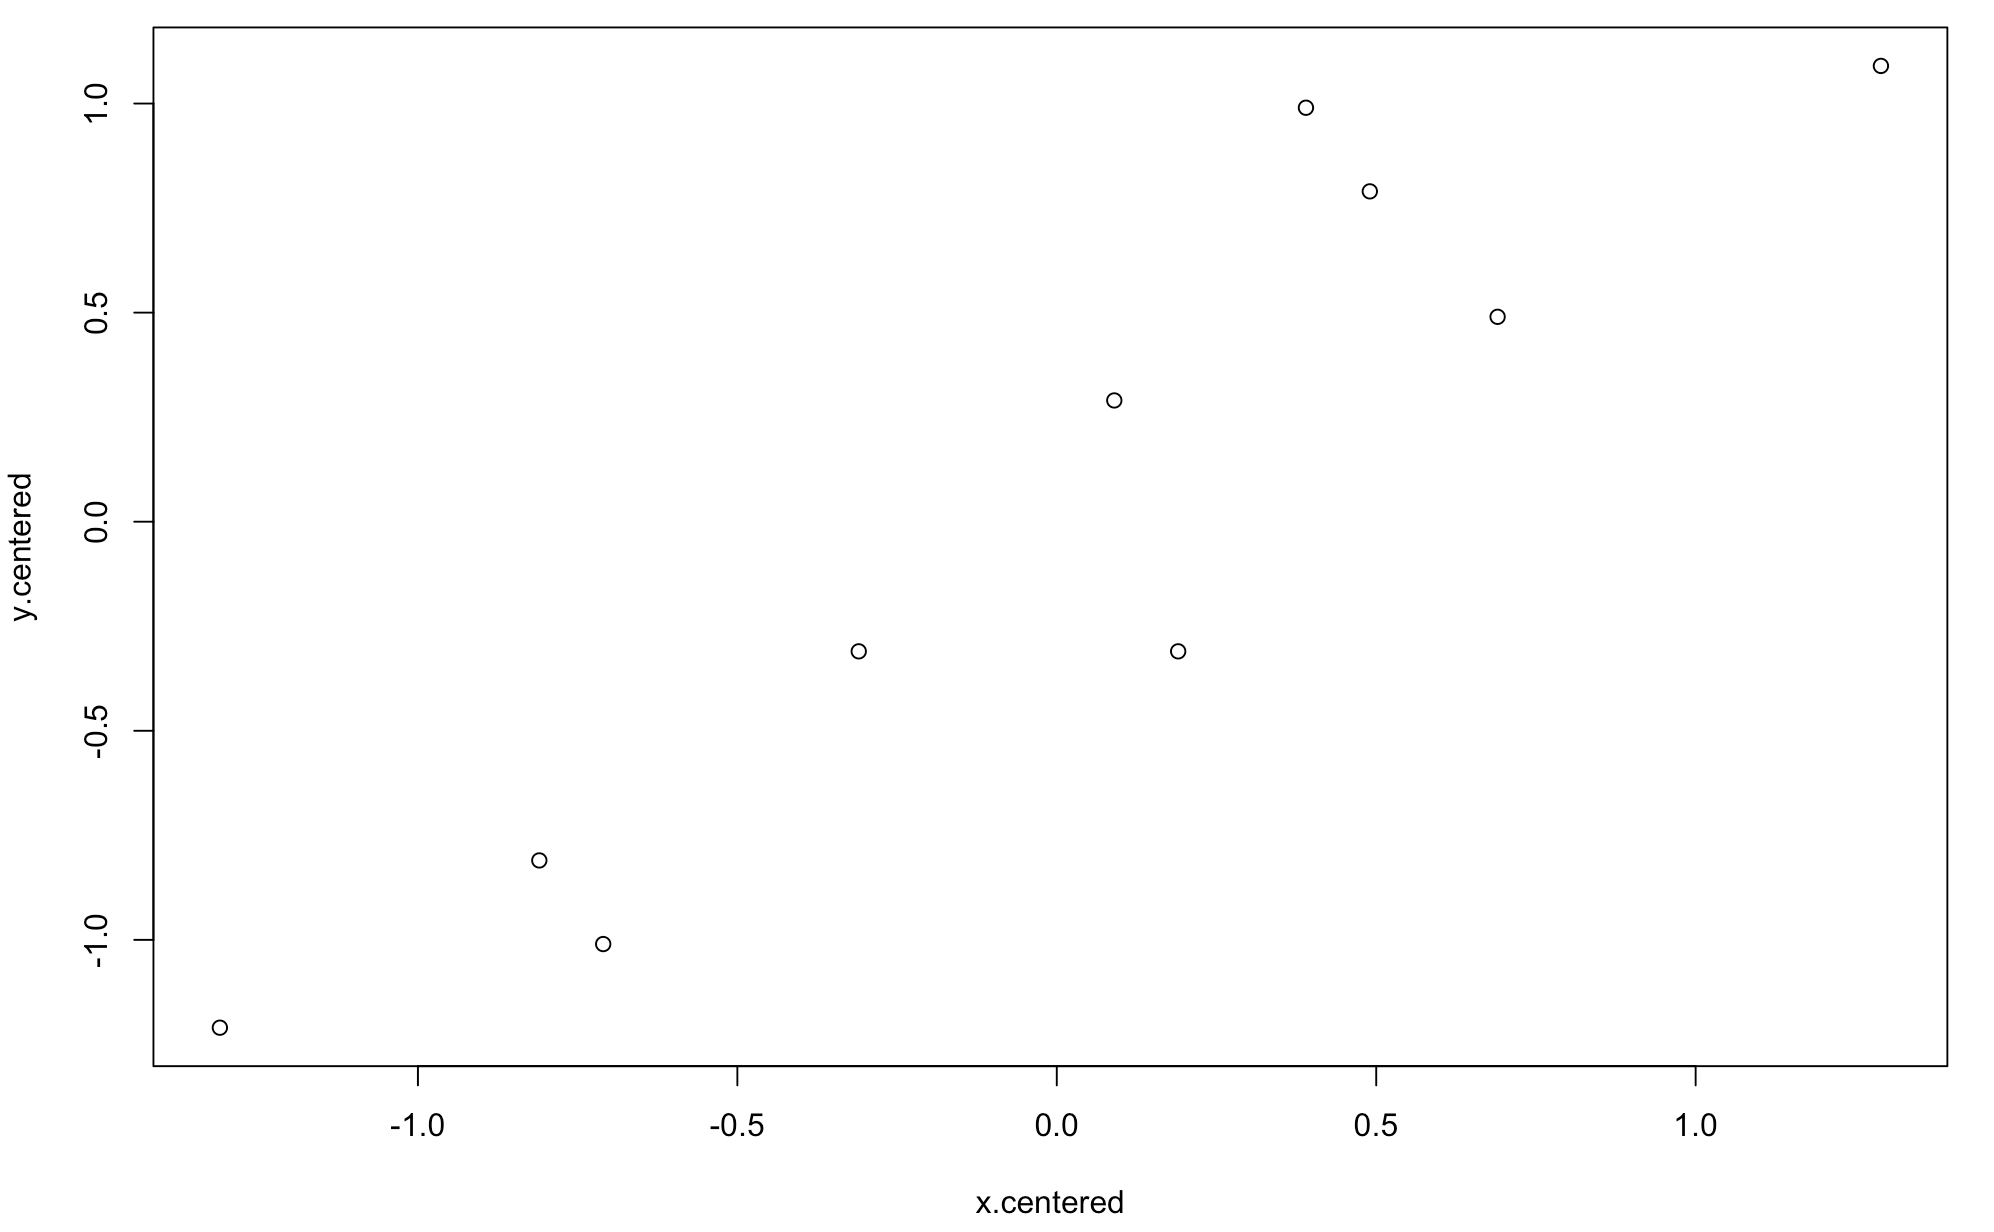
\includegraphics[width=\textwidth]{example1-plot-two-genes-centered}
		\caption{}
		\label{fig:PlotTwoGenesCentered}
	\end{subfigure}
	\begin{subfigure}{0.45\textwidth}
		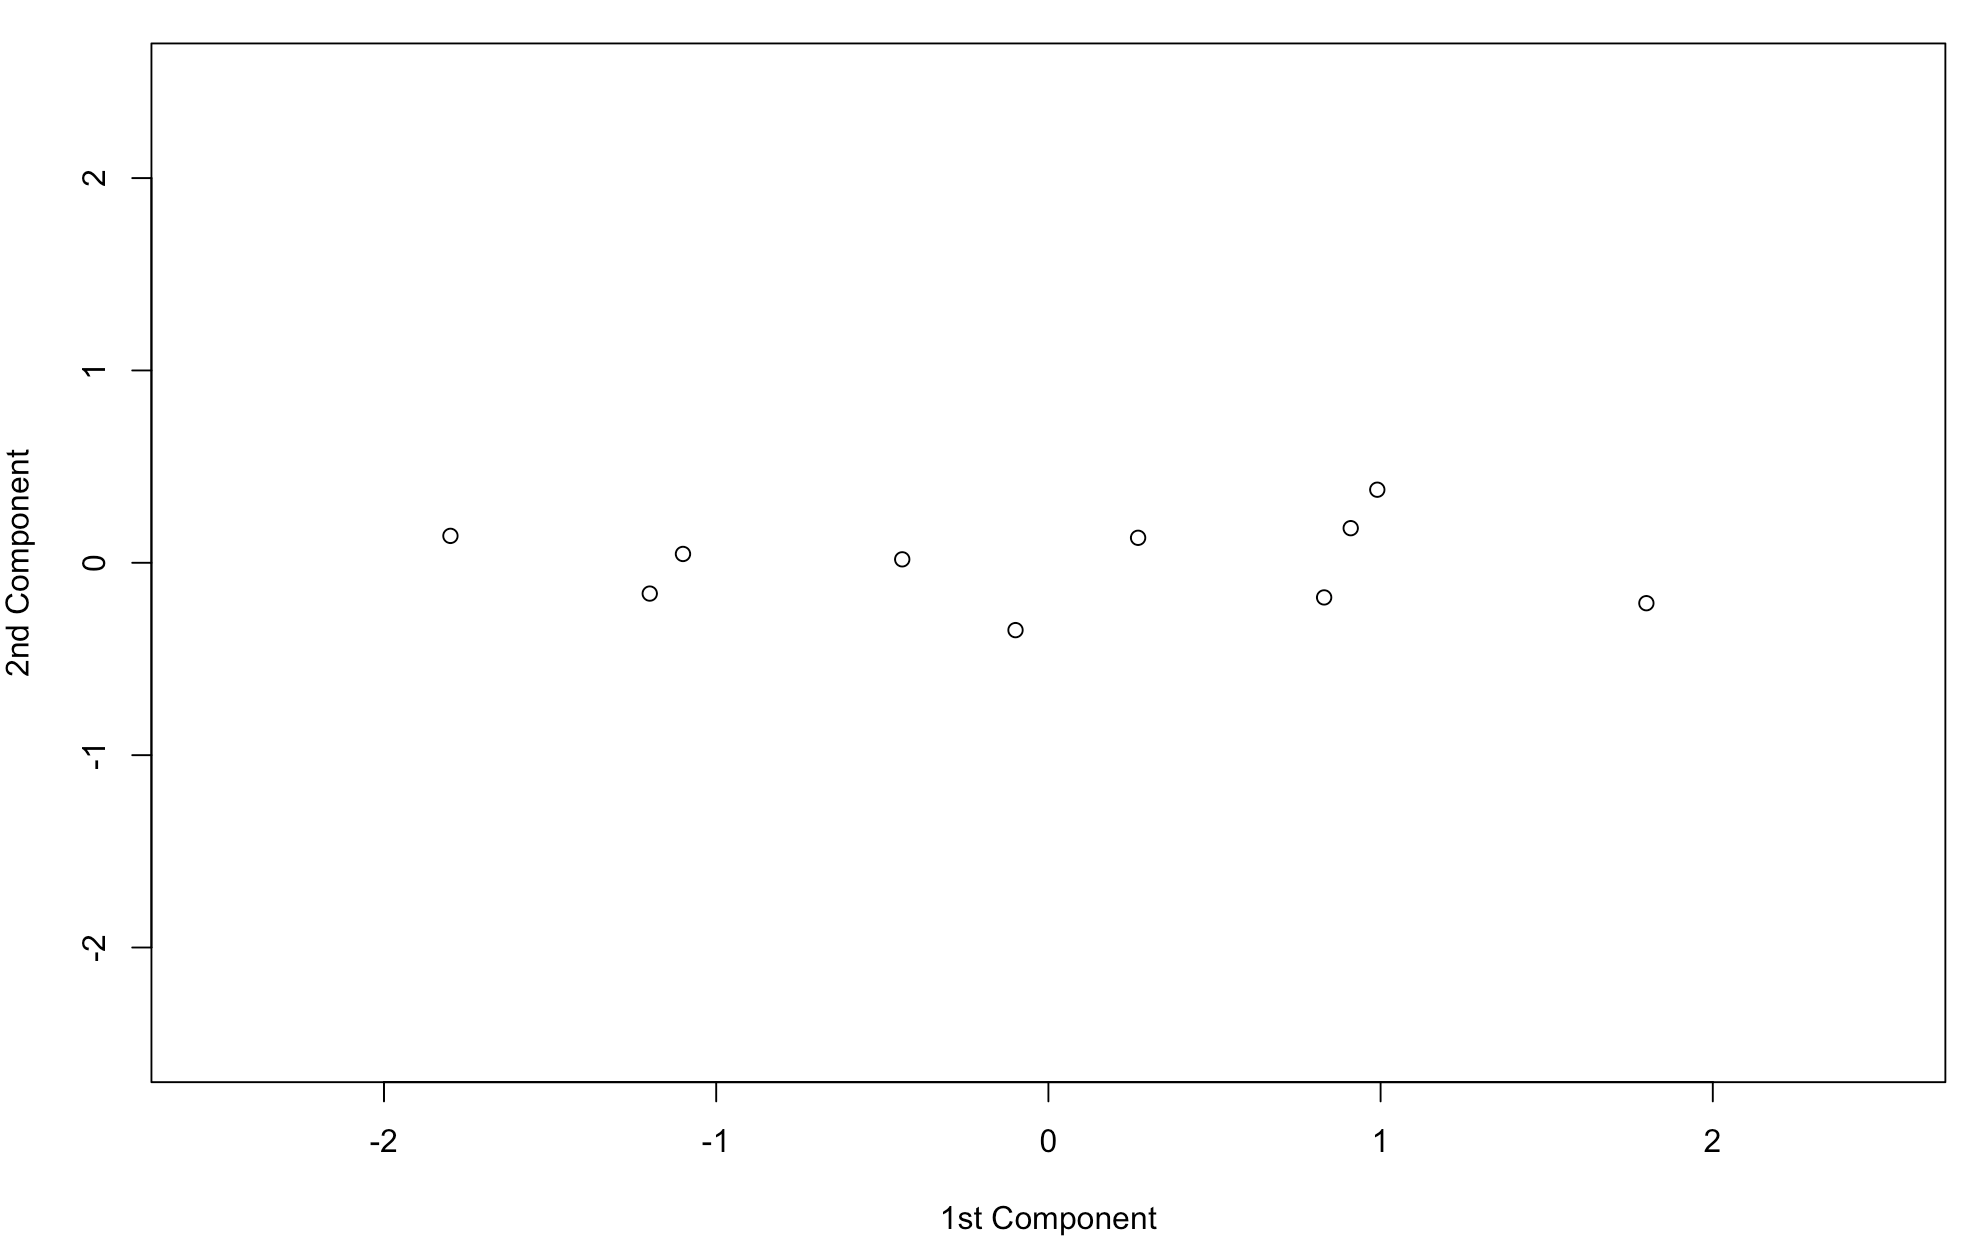
\includegraphics[width=\textwidth]{example1_plot_2PC}
		\caption{}
		\label{fig:PlotTwoGenesNewCoordiantes}
	\end{subfigure}
	\caption{Plot: in (a) shows the expression of two genes, (b) the expression of the same two genes after centering the data (expression has zero mean),  (c) gene expression is plot in the new coordiantes (PCA)}
	\label{fig:PlotData}
\end{figure}


Now, let us calculate the covariance matrix. Covariance matrix for two variables:

\[ \left[ \begin{array}{cc}
      $Cov(x,x)$ & $Cov(x,y)$\\ 
      $Cov(y,x)$ & $Cov(y,y)$
      \end{array} \right]
\]

\noindent and Covariance matrix for our data:
\[
   \left[ \begin{array}{cc}
      0.016 & 0.615 \\ 
      0.615 & 0.716
      \end{array} \right]
\]

The Eigenvalues of this matrix are:  1.284 and 0.0490. Eigenvalues gives the relative variance of the data in the direction defined by the Eigenvectors. From the values we can inferred that most variation is in one direction. To calculate the Eigenvalues in R use type:

\begin{framed}
\begin{verbatim}
	eigen(covariance_matrix)
\end{verbatim}
\end{framed}

The corresponding eigenvector are then placed in a matrix in descending order of eigenvalue:

\[
   \left[ \begin{array}{cc}
	0.6778734 & $-0.7351787$ \\
	0.7351787 & 0.6778734
      \end{array} \right]
\]

The transpose of this Eigenvectos will perform the coordinate transformation:

\[
   W^T = 
   \left[ \begin{array}{cc}
	0.6778734 & 0.7351787 \\
	$-0.7351787$ & 0.6778734
      \end{array} \right]
\]

\noindent This is an orthogonal matrix which performs a rotated-axis coordinate transformation.
We can transform our data matrix so that the data is represented in the new coordinates:  

\[
   D_{PCA} = W^T D
\]

\noindent which in our example is:

\[
   D_{PCA} = 
   \left[ \begin{array}{cc}
	0.6778734 & 0.7351787 \\
	$-0.7351787$ & 0.6778734
   \end{array} \right]
   %
   \left[ \begin{array}{cccccccccc}
      0.69 & $-1.31$ & 0.39 & 0.09 & 1.29 & 0.49 & 0.19 & $-0.81$ & $-0.31$ & $-0.71$ \\
      0.49 & $-1.21$ & 0.99 & 0.29 & 1.09 & 0.79 & $-0.31$ & $-0.81$ & $-0.31$ & $-1.01$
   \end{array} \right]
\]

\[
   =
   %
   \left[ \begin{array}{cccccccccc}
      0.83 & $-1.8$ & 0.99 & 0.27 & 1.8 & 0.91 & $-0.099$ & $-1.1$ & $-0.44$ & $-1.2$ \\
      $-0.18$ & 0.14 & 0.38 & 0.13 & $-0.21$ & 0.18 & $-0.35$ & 0.046 & 0.018 & $-0.16$
   \end{array} \right]
\]


The we can plot our data in the new coordinates, as shown in figure \ref{fig:PlotTwoGenesNewCoordiantes}, where each coordinate is called principal component. 
The first coordinate aligns with the direction in the expression space where has the most variation. Subsequent coordinates would align with directions with descending degrees of variation. This is why we are careful to order according to the size of the eigenvalues.
Thus, PCA is capturing as much variation in the first component as possible, then the same for the second coordinate, and so on.
In the case of our data, all the meaningful variation sees to have been captured with the first coordinate, or the first principal component. Specially compared to the second component which would seem to be random scatter. So we have reduced the dimensionality of our data from two to one. In cases when dealing with thousands of genes, PCA might be able to capture most of the variation of the data in with only two or three principal components. Thus making it easier to visualise it, which is one of the main motivations of performing PCA.


\begin{figure}[!h]
	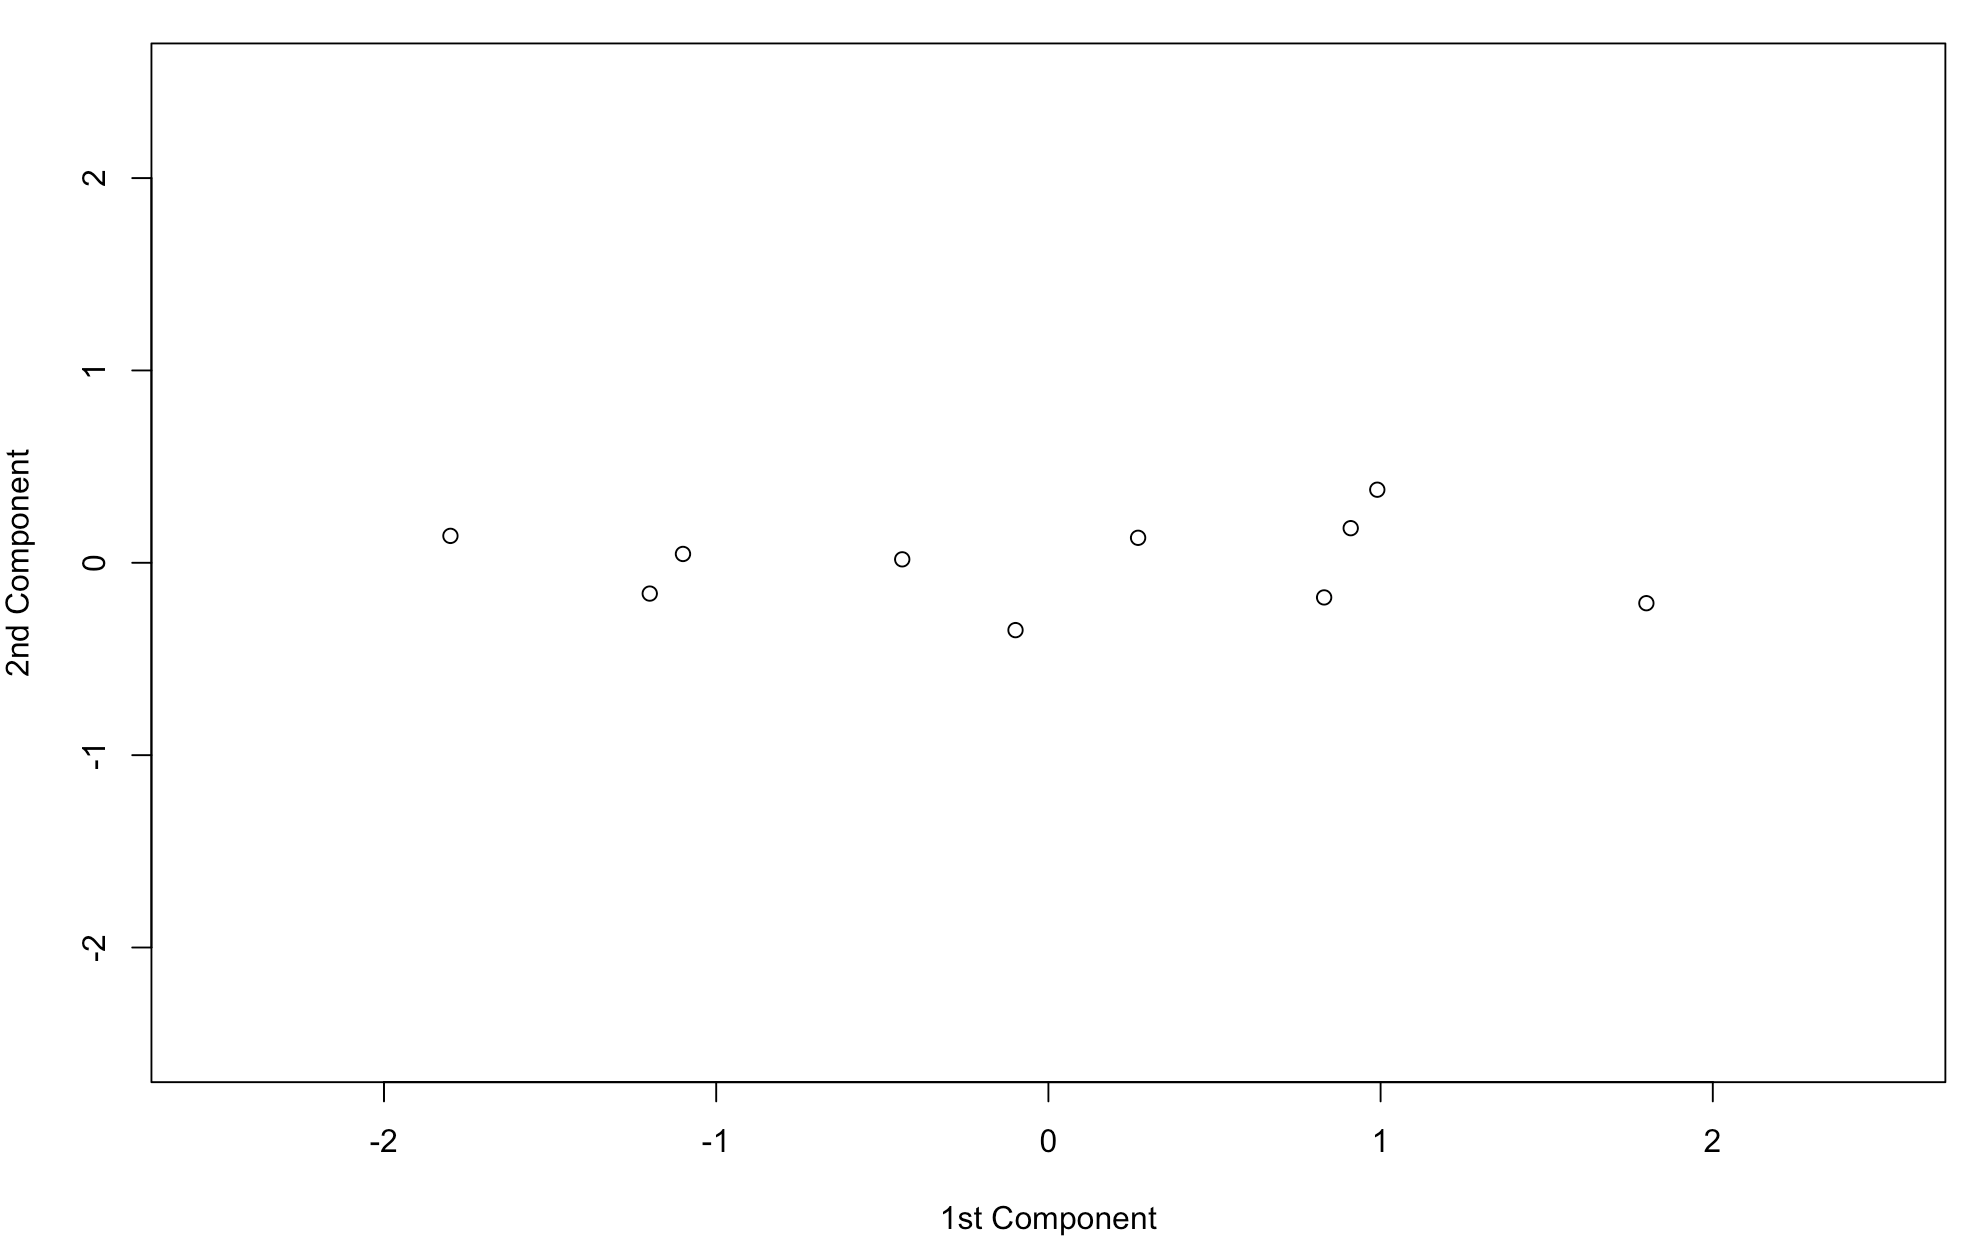
\includegraphics[width=\textwidth]{example1_plot_2PC}
	\caption{Plot of two genes in the new coordinates}
	\label{fig:PlotTwoGenesNewCoordiantes}
\end{figure}




% Example 2: loading example data from file
\paragraph{Example 2: PCA using example data}
\paragraph{}

For this example, we will load a file with gene expression data from a study in fatty liver \cite{Wruck2015}. We will use the stats package in R for computing PCA and will show how to visualise it using the function ggbiplot, which was implemented by Vince Q Vu \cite{Vu2016}. 

%% create a matrix with the expression values from table 1: Example of Expression from Cufflinks
\begin{framed}
\begin{verbatim}
	samples <- c('sample_1', 'sample_2', ..., 'sample_n')
	genes <- c(gene_1, gene_2, ..., gene_m) #numbers
	s1 <- c(gene1_sample1, ..., gene_m_sample_1)
	...
	sn <- c(gene1_sample_n, gene_m_sample_n)

	ExpData <- data.frame(s1, ..., sn)
	colnames(ExpData) <- samples
	rownames(ExpData) <- genes
\end{verbatim}
\end{framed}


Plot using ggbiplot \cite{Vu2016} is shown in figure \ref{fig:PCAFattyLiver}.
The ellipse in the figure represents the normal data ellipse for each group for the details of 68\%. 

\begin{figure}[!h]
	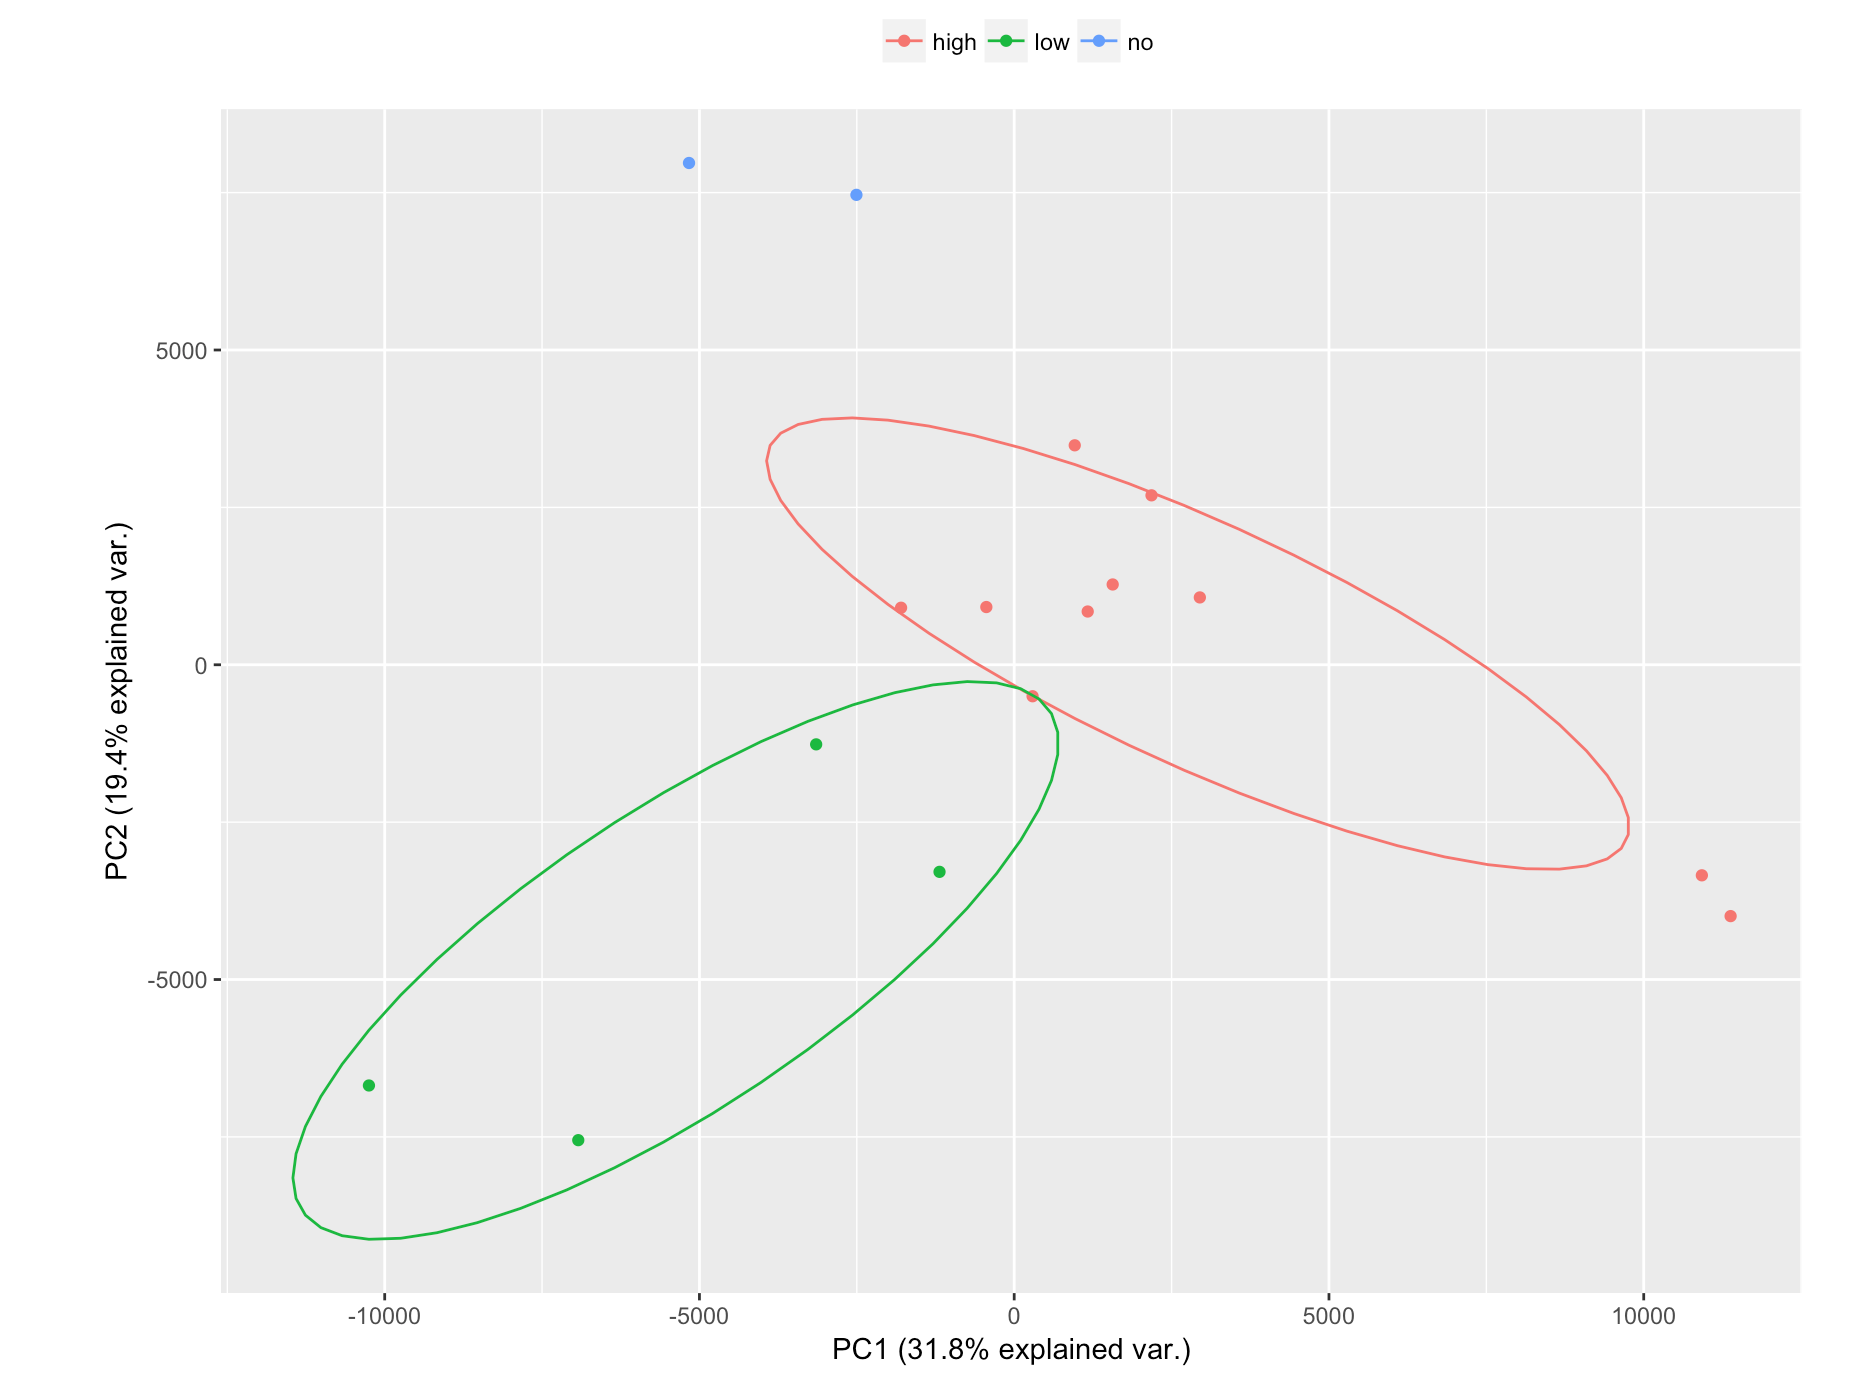
\includegraphics[width=\textwidth]{example2-first2components-fattyLiverData}
	\caption{The first two principal components for gene expression data in a study on Fatty Liver. The plot was generated using the R package ggbiplot \cite{Vu2016}}
	\label{fig:PCAFattyLiver}
\end{figure}


PCA Plot of gene expression data 

Each dot is a gene expression from a sample in each category (class) from a patient, and is coloured by its sub-type

The three axis are the three principal components 
and the numbers represent the percentage of variance that is captured by each component

The first component captures the most variance, whereas the second and third capture only a small percentage

Dots of the same subtype tend to cluster together which means that samples of the same subtype have similar expression profiles.

The distance on the dots on each axis should not be treated equally (as each component captures a different percentage of variance). difference on the first component should be taken into more consideration.



 Random data

Simulated gene expression data by random numbers

This is how a random dataset would look like in a PCA plot:

- dots of different classes mix all together

- the first three components capture almost equal and small variance

- from the plot once would conclude that the different subtypes are not distinct from each other or that subtype has no influence on tumor cell transcriptome



DATA PREPARATION

- Use microarray gene expression data as an example

- Gene expression data is usually stored in a tab delimited text file. The extension of such files could be .csv, .soft, .xls(x), etc. Use Excell of Sublimetext to open and preview the file.

- Gene expression values must be normalised before PCA plotting.


PCA

- We need to transpose the matrix because the function requires the rows of the input matrix to be observations and the columns variable, which means rows to be the gene expression profiles and columns to be the genes.

- There are three outputs to the function:

1. The first output is the coefficient matrix (not used here!)

2. The second output is the scores, which are the transformed coordinates by PCA.

3. The third output, pca variance, stores how much variance each component captures.


Looking into detail on the outputs:

- The first several components capture most variance of the data.

- The score matrix has the same arrangement as expression matrix, which are rows as gene expression profiles and columns are genes. We pick the first three columns, namely the first three components. The first component will be the x-axis, the second to be the y-axis and the third component to be the z-axis.

Running PCA

%in R using prcomp from the stats package
%
%Computing the Principal Components
%
%load the data
%
%normalise data
%log transform (as suggested by xxxxx]
%log.data <- log
%
%Call prcomp with center and scale equal to TRUE to standardise the variables prior PCA



PCA Plot using MultiPEN

Parameters:

gene expression data

groups



In summary, PCA is a method of revealing underling trends in large amounts of data. PCA reduces high dimensional data to just a few principal components which hopefully capture most of the variation of the data and allows inferring meaningful structure.

A new coordinate system is constructed by rotating the axes (each representing a gene). The first new coordinate, or first principal component, is the direction in which the data varies most, then the second component, and so on. PCA allows to select a few new variables which contain most of the variation of the data which can also be visualised.


\subsubsection{Hierarchical Clustering}

Hierarchical Clustering is another way to visualise high dimensional data. 
It clusters observations by distance and builds a hierarchical structure 
It gives more detailed information of the differences among clusters, for example, what genes contributes the most to the differences between two clusters.

Figure: Example of clustergram
The clustergram is made of a heat map in the middle and dendograms in the left and top, with row and column labels on the right and bottom (depending on the number of genes and samples), and a scale bar. 
Each column is a sample expression profile, and each row represents a gene.
The colours suggests relative expression values, where red indicates high expression values and blue indicates low expression values. Ideally, samples of the same type will cluster together


Figure: Example of clustergram of simulated random numbers
No distinct clusters are observed. High and low expression values (red and blue colours) are mixed all together and the sample of the same type are mixed.


Hierarchical clustering uses a distance metric (typically Euclidean but could be correlation, Hamming distance, etc.) between each pair of genes to create a hierarchical tree-like structure of the data. Then it uses a linkage function to calculate the distance between clusters. For more details please see \cite{Clustergram}. 

EXAMPLE USING MULTIPEN


\subsection{Interaction Network}
\subsubsection{Compile the network with Cytoscape}


\part{Part II}
\section{Ranking genes (Feature Selection)} 

Feature selection with MultiPEN from expression leves and network 


\section{Pathway Analysis}

Objective

Steps

Input data
A list of ranked genes. For this session we will use the rankings from feature selection in ExampleOutputs\/MultiPEN\-Rankings\_lambda0.0001.txt.

To run the R script type in the terminal:

Rscript enrichmentGO.R ../ExampleOutputs/MultiPEN\-Rankings\_lambda0.0001.txt output/




% Boxed code
%\begin{framed}
%\begin{verbatim}
%	
%\end{verbatim}
%\end{framed}


%Example to create a list
%List:
%\begin{itemize}
%	\item item 1
%	\item item 2		
%\end{itemize}


%Example to enumerate a list
%\begin{enumerate}	
%	\item enumerated item
%	\item another item
%\end{enumerate}


%Figure resference \autoref{fig:volcanoplot}). 
%
%\begin{figure}[!h]
%	\centering
%	\includegraphics[width=\textwidth]{VolcanoMatrix}
%	\caption{Matrix of volcano plots explore genes that differ significantly between pairs of conditions}
%	\label{fig:volcanoplot}
%\end{figure}

%figure with subfigures
%\begin{figure}[!h]
%	\centering
%	\begin{subfigure}{.3\textwidth}
%		\includegraphics[width=\textwidth]{MAPlotEPS1_8_EPS2_8}
%		\caption{MA for EPS1 and EPS2, 8 hours}
%		\label{fig:MAPlotEPS1_8_EPS2_8}
%	\end{subfigure}
%	\begin{subfigure}{0.3\textwidth}
%		\includegraphics[width=\textwidth]{MAPlotEPS1_8_noEPS_8}
%		\caption{MA for EPS1 and noEPS, 8 hours}
%		\label{fig:MAPlotEPS1_8_noEPS_8}
%	\end{subfigure}
%	\begin{subfigure}{.3\textwidth}
%		\includegraphics[width=\textwidth]{MAPlotEPS2_8_noEPS_8}
%		\caption{MA for EPS2 and noEPS, 8 hours}
%		\label{fig:MAPlotEPS2_8_noEPS_8}
%	\end{subfigure}
%	\caption{Average intensity vs log ratio Plots, for 8 hours}
%	\label{fig:MAPlot_8hours}
%\end{figure}


%See below example of table  \autoref{tab:table1}
%\begin{table}[h]
%	\centering
%	\caption{Example of table 1}
%	\begin{tabular}{c | c | c}
%		\hline
%		column 1 & column 2 & column 3 \\
%		\hline
%		aaaaa  & bbbbbbb & ccccccc \\ 
%		xxxxxxx  & yyyyyyyy & zzzzzzzz \\		
%		\label{tab:table1}
%	\end{tabular}
%\end{table}





\bibliography{references}
\bibliographystyle{plain}

\end{document}  